\documentclass[11pt,a4paper]{article}

% ---------------------------------------------------------------------------
\usepackage[margin=2.2cm]{geometry}
\usepackage[T1]{fontenc}
\usepackage{lmodern}
\usepackage{microtype}
\usepackage{amsmath,amssymb}
\usepackage{booktabs,tabularx}
\usepackage{xcolor}
\usepackage{tikz}
\usetikzlibrary{arrows.meta,positioning,calc,decorations.pathreplacing,patterns,shapes.geometric}
\usepackage{listings}
\usepackage{enumitem}
\usepackage{pifont}
\usepackage[most]{tcolorbox}
\usepackage{caption}
\usepackage{hyperref}
\hypersetup{colorlinks=true,linkcolor=f2cblue,urlcolor=f2cblue,citecolor=f2cblue}

\definecolor{f2cblue}{HTML}{2F6DB5}
\definecolor{f2corange}{HTML}{E07B39}
\definecolor{paddock}{HTML}{CFE3B0}
\definecolor{headland}{HTML}{EADFB8}
\definecolor{canopy}{HTML}{2F6B2F}
\definecolor{bufferc}{HTML}{A0522D}
\definecolor{hltrack}{HTML}{8E5CB8}
\definecolor{codebg}{HTML}{F6F8FA}

\lstset{basicstyle=\ttfamily\small,backgroundcolor=\color{codebg},frame=single,
  rulecolor=\color{black!15},keywordstyle=\color{f2cblue}\bfseries,
  commentstyle=\color{black!55}\itshape,stringstyle=\color{f2corange},
  language=Python,columns=fullflexible,breaklines=true,showstringspaces=false,
  xleftmargin=4pt,xrightmargin=4pt,aboveskip=6pt,belowskip=6pt}

\newtcolorbox{runbox}[1][]{colback=f2cblue!5,colframe=f2cblue,boxrule=0.6pt,
  arc=2pt,left=6pt,right=6pt,top=4pt,bottom=4pt,fonttitle=\bfseries\small,title=#1}
\newtcolorbox{seebox}{colback=paddock!40,colframe=canopy,boxrule=0.6pt,arc=2pt,
  left=6pt,right=6pt,top=4pt,bottom=4pt,fonttitle=\bfseries\small,title=What you should see}
\newtcolorbox{trybox}{colback=f2corange!7,colframe=f2corange,boxrule=0.6pt,arc=2pt,
  left=6pt,right=6pt,top=4pt,bottom=4pt,fonttitle=\bfseries\small,title=Experiment}

\newcommand{\code}[1]{\texttt{\small #1}}
\newcommand{\cell}[1]{\textsf{\bfseries\color{f2cblue}#1}}

\title{\textbf{Optimal Coverage Path Planning for a Paddock with Trees}\\[4pt]
  \large A step-by-step guide to the Fields2Cover Colab notebook}
\author{Companion handout to \code{Fields2Cover\_Paddock\_Trees.ipynb}}
\date{\today}

% ===========================================================================
\begin{document}
\maketitle

\begin{abstract}
\noindent This handout walks you through a Google Colab notebook that uses the open-source library
\emph{Fields2Cover} (F2C, v2.1.1) to plan an optimal coverage path for an agricultural machine.
We first plan a path for an open paddock and then for the same paddock with pinpointed trees.
For every notebook section, the handout gives the underlying mathematics, \emph{what to run},
\emph{what you should see}, and \emph{what to change} to experiment.
No local installation is needed, because everything runs in the cloud.
\end{abstract}

\tableofcontents
\bigskip

% ===========================================================================
\section{Learning objectives}
After this tutorial you will be able to:
\begin{enumerate}[nosep]
  \item explain the four stages of coverage path planning (CPP): headlands, swaths, route and path;
  \item choose a swath direction by minimising an objective function $J(\theta)$;
  \item compare route patterns (boustrophedon, snake, spiral) with an OR-Tools optimised route;
  \item compare Dubins, Reeds--Shepp and continuous-curvature turns for a machine with radius $r_{\min}$;
  \item model trees as buffered obstacles (holes), and plan around them with and without cell decomposition;
  \item validate tree clearance and export the path (CSV/GeoJSON) for QGIS or a guidance terminal.
\end{enumerate}

% ===========================================================================
\section{Opening the notebook in Google Colab}\label{sec:colab}

\begin{runbox}[Steps]
\begin{enumerate}[nosep,leftmargin=*]
  \item Open \href{https://drive.google.com}{Google Drive} and find \code{Fields2Cover\_Paddock\_Trees.ipynb}.
  \item Right-click $\rightarrow$ \emph{Open with} $\rightarrow$ \emph{Google Colaboratory}.
        (If Colab is not listed, choose \emph{Connect more apps} and install it.)
  \item \emph{Runtime $\rightarrow$ Change runtime type}: a standard CPU runtime is enough, and no GPU is needed.
  \item Run the \cell{Part 0} cell. It compiles F2C, which takes about 10--15\,min the first time.
  \item Then choose \emph{Runtime $\rightarrow$ Run all}, or step through the cells with \texttt{Shift+Enter}.
\end{enumerate}
\end{runbox}

\paragraph{Why compile?} F2C is a C++ library with Python bindings generated by SWIG. PyPI only distributes the
\emph{source}, so the setup cell (i)~installs GDAL, GEOS, Eigen, TBB, TinyXML2 and nlohmann-json with \code{apt},
(ii)~downloads the pre-built Google OR-Tools v9.9 C++ release to \code{/opt/or-tools}, and (iii)~builds a wheel from the
\code{v2.1.1} Git tag:
\begin{lstlisting}[language={}]
env CMAKE_PREFIX_PATH=/opt/or-tools \
  pip wheel --no-deps git+https://github.com/Fields2Cover/Fields2Cover.git@v2.1.1
\end{lstlisting}

\paragraph{Faster restarts.} Colab virtual machines are reset after inactivity. If you set
\code{USE\_DRIVE\_CACHE = True}, the cell stores the wheel and the OR-Tools archive in \code{MyDrive/F2C\_cache}, and later
sessions install in under a minute.

% ===========================================================================
\section{Background: the CPP pipeline}\label{sec:theory}

F2C splits CPP into four modules that run one after the other (Fig.~\ref{fig:pipeline}). Each module optimises its own objective.

\begin{figure}[h]
\centering
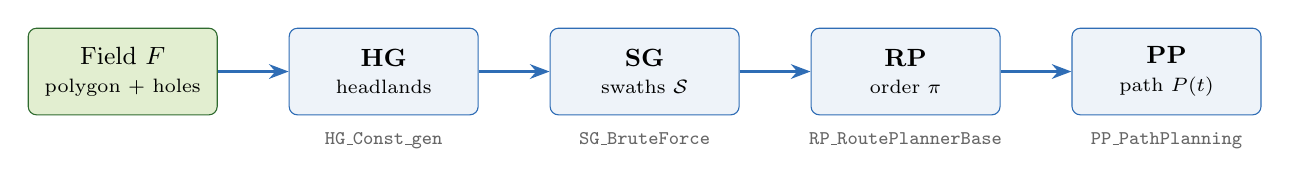
\begin{tikzpicture}[node distance=6mm and 9mm,
  box/.style={draw=f2cblue,fill=f2cblue!8,rounded corners=3pt,minimum width=24mm,
              minimum height=11mm,align=center,font=\small},
  arr/.style={-{Stealth[length=2.5mm]},thick,f2cblue}]
  \node[box,fill=paddock!60,draw=canopy] (F) {Field $F$\\[-1pt]\scriptsize polygon + holes};
  \node[box,right=of F] (HG) {\textbf{HG}\\[-1pt]\scriptsize headlands};
  \node[box,right=of HG] (SG) {\textbf{SG}\\[-1pt]\scriptsize swaths $\mathcal S$};
  \node[box,right=of SG] (RP) {\textbf{RP}\\[-1pt]\scriptsize order $\pi$};
  \node[box,right=of RP] (PP) {\textbf{PP}\\[-1pt]\scriptsize path $P(t)$};
  \foreach \a/\b in {F/HG,HG/SG,SG/RP,RP/PP} \draw[arr] (\a) -- (\b);
  \node[below=1mm of HG,font=\scriptsize\ttfamily,text=black!60] {HG\_Const\_gen};
  \node[below=1mm of SG,font=\scriptsize\ttfamily,text=black!60] {SG\_BruteForce};
  \node[below=1mm of RP,font=\scriptsize\ttfamily,text=black!60] {RP\_RoutePlannerBase};
  \node[below=1mm of PP,font=\scriptsize\ttfamily,text=black!60] {PP\_PathPlanning};
\end{tikzpicture}
\caption{The Fields2Cover pipeline and the Python classes used in the notebook.}
\label{fig:pipeline}
\end{figure}

\subsection{Headlands and swaths}
With machine width $w$, coverage width $w_c$ and a headland of $k$ machine widths, the \emph{mainland} is the eroded field
\begin{equation}
F_{\text{in}} = F \ominus \mathcal B(k\,w),
\end{equation}
where $\ominus$ is erosion (a negative buffer). The ring at $1.5\,w$ is the \emph{headland track} that the route planner uses
to move between swaths. Swaths are parallel lines spaced at $w_c$. For a direction $\theta$ their number is approximately
\begin{equation}
N(\theta)\approx\left\lceil\frac{W_\perp(\theta)}{w_c}\right\rceil,\qquad
\theta^*=\arg\min_{\theta\in[0,\pi)}J(\theta),
\end{equation}
where $W_\perp(\theta)$ is the width of $F_{\text{in}}$ across the driving direction. Every swath costs one turn, so
minimising $N$ (\code{OBJ\_NSwathModified}) usually minimises the non-productive time.

\begin{figure}[h]
\centering
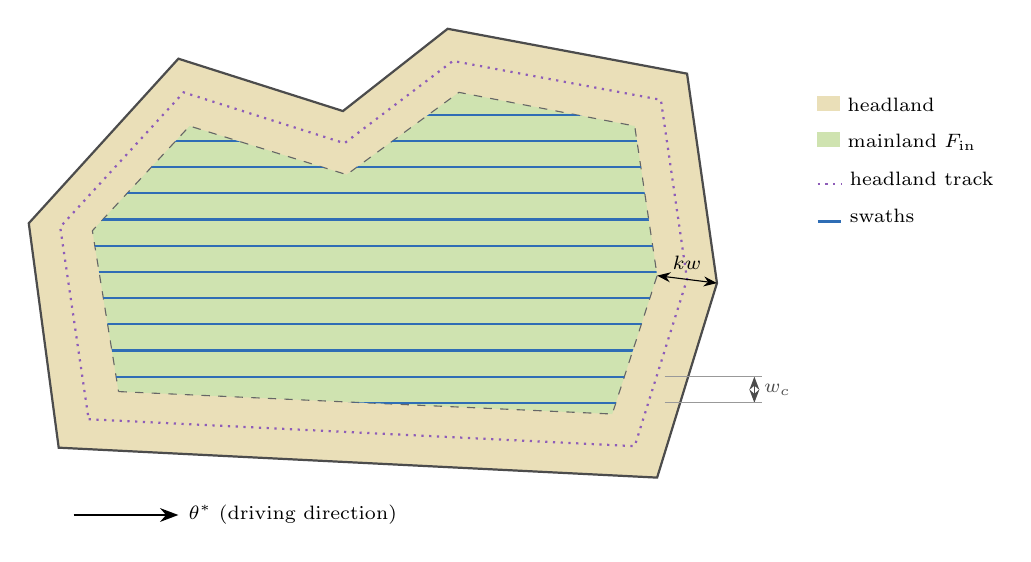
\begin{tikzpicture}[scale=0.95]
  % field
  \fill[headland] (0,0) -- (8,-0.4) -- (8.8,2.2) -- (8.4,5) -- (5.2,5.6) -- (3.8,4.5) -- (1.6,5.2) -- (-0.4,3) -- cycle;
  \draw[thick,black!70] (0,0) -- (8,-0.4) -- (8.8,2.2) -- (8.4,5) -- (5.2,5.6) -- (3.8,4.5) -- (1.6,5.2) -- (-0.4,3) -- cycle;
  % mainland (hand-drawn inset)
  \fill[paddock] (0.8,0.75) -- (7.4,0.45) -- (8.0,2.3) -- (7.7,4.3) -- (5.35,4.75) -- (3.85,3.65) -- (1.75,4.3) -- (0.45,2.9) -- cycle;
  \draw[dashed,black!60] (0.8,0.75) -- (7.4,0.45) -- (8.0,2.3) -- (7.7,4.3) -- (5.35,4.75) -- (3.85,3.65) -- (1.75,4.3) -- (0.45,2.9) -- cycle;
  % headland track
  \draw[hltrack,dotted,thick] (0.4,0.38) -- (7.7,0.02) -- (8.4,2.25) -- (8.05,4.65) -- (5.27,5.17) -- (3.82,4.07) -- (1.67,4.75) -- (0.02,2.95) -- cycle;
  % swaths
  \begin{scope}
    \clip (0.8,0.75) -- (7.4,0.45) -- (8.0,2.3) -- (7.7,4.3) -- (5.35,4.75) -- (3.85,3.65) -- (1.75,4.3) -- (0.45,2.9) -- cycle;
    \foreach \y in {0.6,0.95,...,4.8} \draw[f2cblue,thick] (-1,\y) -- (10,\y);
  \end{scope}
  % dimension of headland
  \draw[{Stealth}-{Stealth}] (8.8,2.2) -- (8.0,2.3) node[midway,above,font=\scriptsize] {$k w$};
  \draw[{Stealth}-{Stealth},black!70] (9.3,0.6) -- (9.3,0.95) node[midway,right,font=\scriptsize] {$w_c$};
  \draw[black!40] (8.1,0.6) -- (9.4,0.6) (8.1,0.95) -- (9.4,0.95);
  % theta
  \draw[-{Stealth},thick] (0.2,-0.9) -- (1.6,-0.9) node[right,font=\scriptsize] {$\theta^*$ (driving direction)};
  % legend
  \node[font=\scriptsize,anchor=west] at (10.0,4.6) {\tikz\fill[headland] (0,0) rectangle (0.3,0.2); headland};
  \node[font=\scriptsize,anchor=west] at (10.0,4.1) {\tikz\fill[paddock] (0,0) rectangle (0.3,0.2); mainland $F_{\text{in}}$};
  \node[font=\scriptsize,anchor=west] at (10.0,3.6) {\tikz\draw[hltrack,dotted,thick] (0,0.1) -- (0.3,0.1); headland track};
  \node[font=\scriptsize,anchor=west] at (10.0,3.1) {\tikz\draw[f2cblue,thick] (0,0.1) -- (0.3,0.1); swaths};
\end{tikzpicture}
\caption{Headland, mainland, headland track and swaths for a paddock like the one in the notebook.}
\label{fig:geom}
\end{figure}

\subsection{Routes and turns}
The route planner chooses the order $\pi$ and the direction of the swaths. It minimises the headland travel between consecutive swaths,
\begin{equation}
\min_{\pi}\sum_{j=1}^{N-1} d_{hl}\bigl(\text{end}(s_{\pi_j}),\text{start}(s_{\pi_{j+1}})\bigr),
\end{equation}
with OR-Tools. The path planner then joins the swaths with turns that respect the curvature limits
\begin{equation}
|\kappa|\le\kappa_{\max}=\frac1{r_{\min}},\qquad \left|\frac{d\kappa}{ds}\right|\le\sigma_{\max}\ \text{(continuous curvature)}.
\end{equation}

\begin{figure}[h]
\centering
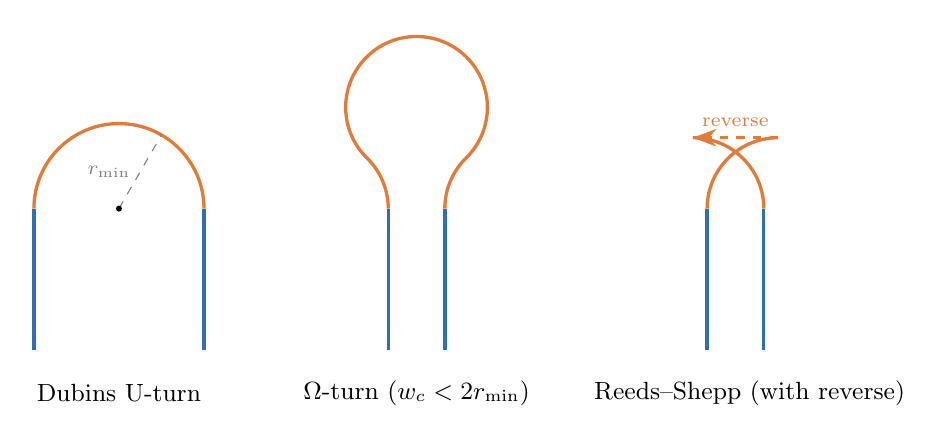
\begin{tikzpicture}[scale=0.9]
  % Dubins U-turn (bulb)
  \draw[f2cblue,very thick] (0,-2) -- (0,0);
  \draw[f2cblue,very thick] (2.4,0) -- (2.4,-2);
  \draw[f2corange,very thick] (0,0) arc (180:0:1.2);
  \draw[dashed,black!50] (1.2,0) -- ++(60:1.2) node[midway,left,font=\scriptsize] {$r_{\min}$};
  \fill (1.2,0) circle (1.2pt);
  \node[font=\small] at (1.2,-2.6) {Dubins U-turn};
  % omega turn when spacing < 2r
  \begin{scope}[xshift=5cm]
    \draw[f2cblue,very thick] (0,-2) -- (0,0);
    \draw[f2cblue,very thick] (0.8,0) -- (0.8,-2);
    % left arc (c=(-1,0)) -> right arc (c=(0.4,1.428)) -> left arc (c=(1.8,0)), r = 1
    \draw[f2corange,very thick] (0,0) arc (0:45.6:1.0) arc (225.6:-45.6:1.0) arc (134.4:180:1.0);
    \node[font=\small] at (0.4,-2.6) {$\Omega$-turn ($w_c<2r_{\min}$)};
  \end{scope}
  % Reeds-Shepp with reverse
  \begin{scope}[xshift=9.5cm]
    \draw[f2cblue,very thick] (0,-2) -- (0,0);
    \draw[f2cblue,very thick] (0.8,0) -- (0.8,-2);
    % forward right arc -> straight reverse -> forward right arc, r = 1
    \draw[f2corange,very thick] (0,0) arc (180:90:1.0);
    \draw[f2corange,very thick,dashed,-{Stealth}] (1,1) -- (-0.2,1) node[above,midway,font=\scriptsize] {reverse};
    \draw[f2corange,very thick] (-0.2,1) arc (90:0:1.0);
    \node[font=\small] at (0.6,-2.6) {Reeds--Shepp (with reverse)};
  \end{scope}
\end{tikzpicture}
\caption{Turn shapes. When the swath spacing is smaller than $2r_{\min}$, a forward-only machine needs a wide $\Omega$-turn.
Reeds--Shepp paths allow reversing.}
\label{fig:turns}
\end{figure}

The path length and the field efficiency are
\begin{equation}
L=\sum_i L_{\text{swath},i}+\sum_j L_{\text{turn},j},\qquad
\eta=\frac{\sum_i L_{\text{swath},i}}{L},\qquad
T=\frac{L_{\text{swath}}}{v_{\text{cruise}}}+\frac{L_{\text{turn}}}{v_{\text{turn}}}.
\end{equation}

\subsection{Trees as obstacles}
Tree $i$ has a trunk at $\mathbf t_i$ and a canopy radius $r_i$. With a safety margin $m$ its no-go zone and the workable field are
\begin{equation}
B_i=\{\mathbf p:\lVert\mathbf p-\mathbf t_i\rVert\le r_i+m\},\qquad F'=F\setminus\textstyle\bigcup_i B_i .
\end{equation}
Each $B_i$ is a \emph{hole} (an interior ring) of the field polygon. Eroding $F'$ dilates every hole, so a headland of width $kw$
appears around each tree (Fig.~\ref{fig:tree}):
\begin{equation}
F'_{\text{in}}=\bigl(F\ominus\mathcal B(kw)\bigr)\setminus\textstyle\bigcup_i\bigl(B_i\oplus\mathcal B(kw)\bigr).
\end{equation}

\begin{figure}[h]
\centering
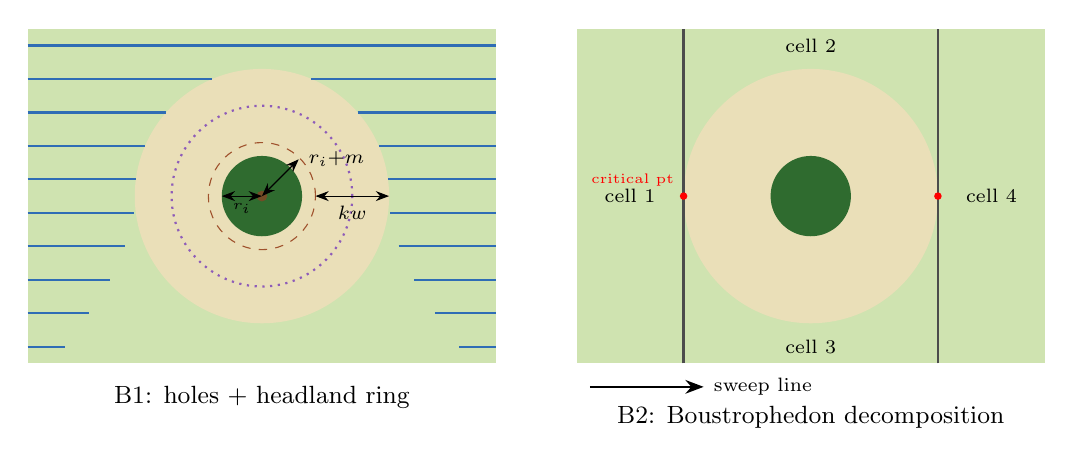
\begin{tikzpicture}[scale=0.85]
  % left: tree + headland + swaths split
  \fill[paddock] (-3.5,-2.5) rectangle (3.5,2.5);
  \fill[headland] (0,0) circle (1.9);
  \draw[hltrack,dotted,thick] (0,0) circle (1.35);
  \draw[bufferc,dashed] (0,0) circle (0.8);
  \fill[canopy] (0,0) circle (0.6);
  \fill[brown!60!black] (0,0) circle (0.08);
  \begin{scope}
    \clip (-3.5,-2.5) rectangle (3.5,2.5);
    \foreach \y in {-2.25,-1.75,...,2.25} {
      \pgfmathsetmacro{\h}{(1.9^2-\y^2)}
      \ifdim \h pt>0pt
        \pgfmathsetmacro{\xx}{sqrt(\h)}
        \draw[f2cblue,thick] (-3.5,\y) -- (-\xx,\y);
        \draw[f2cblue,thick] (\xx,\y) -- (3.5,\y);
      \else
        \draw[f2cblue,thick] (-3.5,\y) -- (3.5,\y);
      \fi
    }
  \end{scope}
  \draw[{Stealth}-{Stealth}] (0,0) -- (-0.6,0) node[pos=0.5,below=-1pt,font=\tiny] {$r_i$};
  \draw[{Stealth}-{Stealth}] (0,0) -- (0.55,0.55) node[right,font=\scriptsize] {$r_i{+}m$};
  \draw[{Stealth}-{Stealth}] (0.8,0) -- (1.9,0) node[midway,below,font=\scriptsize] {$kw$};
  \node[font=\small] at (0,-3) {B1: holes + headland ring};
  % right: boustrophedon decomposition
  \begin{scope}[xshift=8.2cm]
    \fill[paddock] (-3.5,-2.5) rectangle (3.5,2.5);
    \fill[headland] (0,0) circle (1.9);
    \fill[canopy] (0,0) circle (0.6);
    \draw[thick,black!70] (-1.9,-2.5) -- (-1.9,2.5) (1.9,-2.5) -- (1.9,2.5);
    \node[font=\scriptsize] at (-2.7,0) {cell 1};
    \node[font=\scriptsize] at (0,1.95+0.3) {cell 2};
    \node[font=\scriptsize] at (0,-1.95-0.3) {cell 3};
    \node[font=\scriptsize] at (2.7,0) {cell 4};
    \fill[red] (-1.9,0) circle (1.6pt) (1.9,0) circle (1.6pt);
    \node[font=\tiny,red,anchor=south east] at (-1.9,0) {critical pt};
    \draw[-{Stealth},thick] (-3.3,-2.85) -- (-1.6,-2.85) node[right,font=\scriptsize] {sweep line};
    \node[font=\small] at (0,-3.3) {B2: Boustrophedon decomposition};
  \end{scope}
\end{tikzpicture}
\caption{Left: a tree becomes a hole of radius $r_i+m$, with a headland ring of width $kw$ around it. Swaths stop at the ring.
Right: Boustrophedon decomposition cuts the field into cells at the critical points of the obstacle.}
\label{fig:tree}
\end{figure}

% ===========================================================================
\section{Walkthrough of the notebook}

\subsection*{Part 2 --- Configuration and helpers}
\begin{runbox}[Run]
The \code{CONFIG} cell, then the three helper cells (geometry, plotting, metrics).
\end{runbox}
Every tunable value is in one dictionary:
\begin{lstlisting}
CONFIG = dict(paddock=[(0,0),(410,-25),...], width=6.0, cov_width=6.0,
              min_turn_radius=6.0, cruise_vel=2.5, turn_vel=1.2,
              headland_factor=3.0, trees=[(105,70,7.0),...], tree_margin=3.0)
\end{lstlisting}
The helpers convert F2C geometries to \emph{shapely} through WKT (\code{to\_shapely(g)}). This allows clean matplotlib figures with
mowing-stripe coverage, colour-coded path sections, tree glyphs, a scale bar and a north arrow.

% ---------------------------------------------------------------------------
\subsection*{Part A --- Open paddock}

\subsubsection*{A.1 Field and machine}
\begin{lstlisting}
field = f2c.Cells(f2c.Cell(make_ring(CONFIG["paddock"])))
robot = f2c.Robot(W, WC); robot.setMinTurningRadius(6.0)
\end{lstlisting}
\begin{seebox}A $\approx$14\,ha irregular paddock with numbered vertices. Note the concave notch on the northern edge.\end{seebox}

\subsubsection*{A.2 Headland width from the turn geometry}
With \code{headland\_factor="auto"}, $k$ follows from the $\Omega$-turn depth $D_\Omega$ (Section~\ref{sec:improve}).
\begin{lstlisting}
const_hl = f2c.HG_Const_gen()
mid_hl = const_hl.generateHeadlands(field, 0.5 * k * W)   # headland track
no_hl  = const_hl.generateHeadlands(field, k * W)         # mainland
\end{lstlisting}
\begin{seebox}The headland band, the mainland, and the dotted headland rounds that are driven last.\end{seebox}

\subsubsection*{A.3 Optimal swath angle} The notebook sweeps $\theta$ in steps of $1^\circ$ with
\code{bf.computeCostOfAngle(obj, $\theta$, w\_c, cell)}, plots $J(\theta)$ in Cartesian and polar form, and then calls \code{generateBestSwaths}.
\begin{trybox}Change the objective to \code{OBJ\_SwathLength()}. Is $\theta^*$ the same?\end{trybox}

\subsubsection*{A.4 Route from the gate} The boustrophedon, snake and spiral patterns are compared with the OR-Tools route, which
starts and ends at the gate (\code{route\_with\_gate}).
\begin{seebox}A $2\times2$ panel. Each title shows the length, the distance driven over the crop and the distance driven outside the paddock.\end{seebox}

\subsubsection*{A.5 Feasible turns} The four turn models are shown on a zoom. \code{best\_path} keeps whichever of Dubins-CC and
Reeds--Shepp-HC is faster once reversals and driving outside the paddock are penalised.
\begin{trybox}Set \code{allow\_reverse = False}. How many metres are now driven outside the paddock?\end{trybox}

% ---------------------------------------------------------------------------
\subsection*{Part B --- Paddock with trees}
The notebook first explains why a naïve tree workflow is poor (Section~\ref{sec:improve}), then compares three strategies.

\subsubsection*{B.1 Pinpointing} Trees are triples $(x,y,r)$. Set \code{random\_trees = N} to scatter $N$ random, well-separated trees.

\subsubsection*{B.2 Strategy B1: holes}
\begin{lstlisting}
field_B = f2c.Cells(f2c.Cell(make_ring(CONFIG["paddock"])))
for (x, y, r) in TREES:
    field_B.addRing(0, make_ring(circle_coords(x, y, r + M)))
\end{lstlisting}
Headland rings appear around every tree, swaths stop at them, and the route from the gate uses all the headland tracks.

\subsubsection*{B.3 Strategy B2: decomposition}
\begin{lstlisting}
decomp = f2c.DECOMP_Boustrophedon(); decomp.setSplitAngle(best_angle)
decomp_cells = decomp.decompose(mid_hl_B)
no_hl_B2 = f2c.HG_Corridor_gen().generateHeadlands(decomp_cells, 0.5 * k * W)
\end{lstlisting}
The block is wrapped in \code{try/except}. If the decomposition fails, B1 and B3 still run.

\subsubsection*{B.4 Strategy B3: drive around} \code{make\_drive\_around(track\_A, TREES, ...)} adds a detour to each Part~A swath that crosses a tree
(Fig.~\ref{fig:detour}). It reports the extra distance, the maximum curvature (which must stay at or below $1/r_{\min}$), and any trees whose detour did not fit.
\begin{seebox}A zoom on the largest tree: without section control an orange overlap ring appears. With section control only small red wings
beside the tree are left unsprayed.\end{seebox}

\subsubsection*{B.5 Visual comparison} The B1, B2 and B3 paths side by side, with distance, time and metres driven over the crop.

% ---------------------------------------------------------------------------
\subsection*{Part C --- Compare, validate, export}
\subsubsection*{C.1 Scoreboard} One table and bar charts cover A, B1, B2 and B3:
\begin{itemize}[nosep]
  \item time, turns and reversals
  \item metres over the crop and outside the paddock
  \item missed and overlap \% with and without section control
  \item product saved
\end{itemize}
The recommended strategy is chosen automatically.

\subsubsection*{C.2 Coverage maps} A $2\times4$ grid of application-count maps (red = missed, green = once, orange = overlap) without and with section control.

\subsubsection*{C.3 Best path and clearance} For every tree the notebook computes
\begin{equation}
\delta_i=\min_t\lVert P(t)-\mathbf t_i\rVert-r_i-\tfrac{w}{2}
\end{equation}
and asserts $\delta_i>0$. An animation of the machine follows.

\subsubsection*{C.4 Export} The path is saved as a CSV (segment, kind, x, y) and as a GeoJSON (paddock, gate, trees, path pieces). The scoreboard is saved as \code{scenario\_comparison.csv}.
For real paddocks, use \code{transformToUTM} before planning and \code{transformToPrevCRS} afterwards (both in \code{f2c.Transform}).

% ===========================================================================
\section{Diagnosing and improving the tree path}\label{sec:improve}

The first version of the notebook gave a poor path around the trees: about 17\,km and 2.4\,h for 14\,ha. Version~2 fixes the causes and adds a third strategy.

\subsection{Why the path was poor}
\begin{enumerate}[nosep]
  \item \textbf{$\Omega$-loops.} With $w_c=6$\,m $<2r_{\min}=12$\,m, a forward-only U-turn cannot join neighbouring swaths, so every turn became a
        bulb (Fig.~\ref{fig:turns}). Its depth into the headland is
        \begin{equation}
        D_\Omega=r_{\min}+\sqrt{4r_{\min}^2-\left(r_{\min}+\tfrac{w_c}{2}\right)^2},\qquad
        k=\max\!\left(3,\left\lceil\frac{D_\Omega+w/2}{w}\right\rceil\right),
        \end{equation}
        which is how \code{headland\_factor="auto"} chooses $k$. Reeds--Shepp HC turns (\code{allow\_reverse=True}) replace the bulb with a three-point turn.
  \item \textbf{Island headlands.} The headland ring around each tree is not connected to the outer headland, so travel between them became straight hops across the crop.
        This is now reported as \emph{over crop [m]}.
  \item \textbf{Fragmented swaths.} Each tree cut 3--5 swaths in two, and every fragment needed its own turns.
  \item \textbf{Weak search, no gate.} The route search stopped at OR-Tools' first solution, and the route had no fixed start.
\end{enumerate}

\subsection{Gate and route search}
\begin{lstlisting}
rp = f2c.RP_RoutePlannerBase()
rp.setStartAndEndPoint(gate_point(mid_hl))          # gate projected on the headland track
route = rp.genRoute(mid_hl, swaths, False, 1e-4, True, 30, True)   # 30 s guided local search
\end{lstlisting}

\subsection{Strategy B3: drive around the trees}
B3 keeps the open-paddock swaths and route, and splices a detour into each swath that crosses a tree (Fig.~\ref{fig:detour}).
The clearance radius is $R=\max(r_i+m+\tfrac w2,\,r_{\min})$ and the fillet radius is $\rho=r_{\min}$.
Take a frame with the tree at the origin and the swath along $y=a$, where $|a|<R$. Then
\begin{equation}
x_f=\sqrt{(R+\rho)^2-(a+\rho)^2},\qquad C_{1,2}=(\mp x_f,\ a+\rho),\qquad T_{1,2}=\tfrac{R}{R+\rho}\,C_{1,2},
\end{equation}
and the path runs straight $\to$ arc$(\rho)$ $\to$ arc$(R)$ $\to$ arc$(\rho)$ $\to$ straight, with $|\kappa|\le 1/r_{\min}$ throughout.

\begin{figure}[h]
\centering
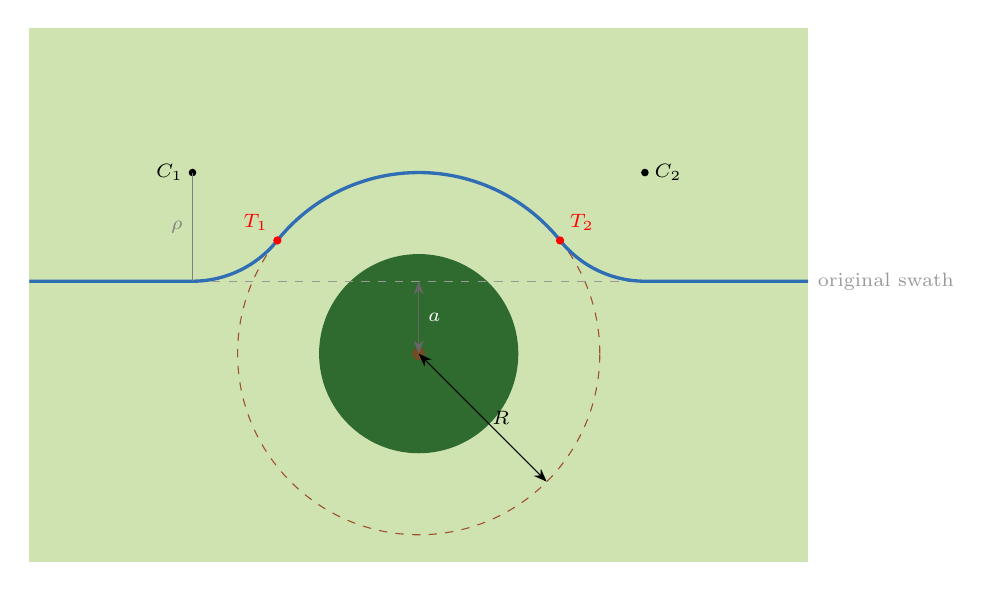
\begin{tikzpicture}[scale=1.15]
  \fill[paddock] (-4.3,-2.3) rectangle (4.3,3.6);
  \draw[dashed,bufferc] (0,0) circle (2);
  \fill[canopy] (0,0) circle (1.1);
  \fill[brown!60!black] (0,0) circle (0.07);
  \draw[black!40,dashed] (-4.3,0.8) -- (4.3,0.8) node[right,font=\scriptsize] {original swath};
  \draw[f2cblue,very thick] (-4.3,0.8) -- (-2.498,0.8) arc[start angle=-90,end angle=-38.68,radius=1.2]
        arc[start angle=141.32,end angle=38.68,radius=2] arc[start angle=-141.32,end angle=-90,radius=1.2] -- (4.3,0.8);
  \fill (-2.498,2.0) circle (1.2pt) node[left,font=\scriptsize] {$C_1$};
  \fill (2.498,2.0) circle (1.2pt) node[right,font=\scriptsize] {$C_2$};
  \draw[black!50] (-2.498,2.0) -- (-2.498,0.8) node[midway,left,font=\scriptsize] {$\rho$};
  \draw[{Stealth}-{Stealth}] (0,0) -- (1.414,-1.414) node[midway,right,font=\scriptsize] {$R$};
  \draw[{Stealth}-{Stealth},black!60] (0,0) -- (0,0.8) node[midway,right,font=\scriptsize,text=white] {$a$};
  \fill[red] (-1.561,1.25) circle (1.3pt) node[above left,font=\scriptsize] {$T_1$};
  \fill[red] (1.561,1.25) circle (1.3pt) node[above right,font=\scriptsize] {$T_2$};
\end{tikzpicture}
\caption{B3 detour: the swath (blue) leaves the straight line on a fillet of radius $\rho=r_{\min}$, circles the tree at clearance $R$, and rejoins the line on a second fillet.}
\label{fig:detour}
\end{figure}

\subsection{Section control}
F2C assumes the implement is fully on along swaths. The notebook adds a raster simulator in which the boom is split into $n_s$ sections.
Section $j$ is on when most of its footprint lies over target ground $F'$ that has not yet been covered:
\begin{equation}
\text{on}_j(t)=\mathbf 1\!\left[\frac{|S_j(t)\cap F'\cap U(t)|}{|S_j(t)|}\ge\tfrac12\right],\qquad
M=\frac{|\{c=0\}\cap F'|}{|F'|},\qquad O=\frac{|\{c\ge2\}\cap F'|}{|F'|},
\end{equation}
where $c$ is the number of passes that applied product to a cell, $M$ is the missed share and $O$ is the overlap share.
The notebook reports $M$, $O$ and the product saved, $1-\int c_{\text{SC}}/\int c_{\text{no SC}}$, for every strategy (Part~C).

% ===========================================================================
\section{Exercises}
\begin{enumerate}
  \item \textbf{Gate.} Move \code{gate} to another paddock vertex. How much do the distance and time change?
  \item \textbf{Skip rows.} Set \code{width = cov\_width = 12} so that $w_c\ge 2r_{\min}$. Do the $\Omega$-loops disappear, and how does $k$ change?
  \item \textbf{Sections.} Compare \code{n\_sections} $=1,3,6,12$. Plot the product saved against $n_s$.
  \item \textbf{Turning radius.} Plot the total length $L$ against $r_{\min}\in\{3,6,9,12\}$\,m for the four turn models.
  \item \textbf{Headland factor.} Derive a lower bound for $k$ so that a U-turn fits in the headland, assuming
        $w_c\ge 2r_{\min}$. Hint: the turn bulges $r_{\min}$ beyond the swath end and the machine is $w$ wide.
        Check your bound in the notebook.
  \item \textbf{Tree density.} Increase \code{random\_trees} from 5 to 25. Plot $\eta$ against the number of trees for B1 and B2.
        Where do the curves cross?
  \item \textbf{Clusters.} Move two trees so that $\lVert\mathbf t_i-\mathbf t_j\rVert<r_i+r_j+2m+2kw$. Explain the merged headland island.
  \item \textbf{Real data.} Replace the synthetic paddock with a GPS boundary and tree points from a drone survey.
\end{enumerate}

% ===========================================================================
\section{Troubleshooting}
\begin{tabularx}{\linewidth}{@{}lX@{}}
\toprule
\textbf{Symptom} & \textbf{Fix}\\
\midrule
\code{find\_package(ortools)} fails & Check that \code{/opt/or-tools/lib/cmake/ortools} exists, then re-run Part 0.\\
\code{ImportError: libortools.so} & Run \code{!ldconfig}, then \emph{Runtime $\rightarrow$ Restart session}.\\
F2C disappears after a break & The Colab VM was recycled. Set \code{USE\_DRIVE\_CACHE = True}.\\
Tree-buffer assertion (B.1) & Move the tree inwards or reduce \code{tree\_margin}.\\
Decomposition error (B.3) & Try another split angle. B1 and B3 still run.\\
``Unresolved trees'' in B3 & The detour does not fit (tree near a swath end or the boundary). Move the tree or use B1.\\
Kernel restarts, no error & A C++ crash from a dangling reference. Copy items out with \code{.clone()}.\\
Clearance assertion (C.3) & Increase \code{tree\_margin} or \code{headland\_factor}.\\
\bottomrule
\end{tabularx}

% ===========================================================================
\section*{References}
\begin{enumerate}[label={[\arabic*]},nosep]
  \item G.~Mier, J.~Valente, S.~de~Bruin, ``Fields2Cover: An open-source coverage path planning library for unmanned
        agricultural vehicles,'' \emph{IEEE Robotics and Automation Letters}, 8(4):2166--2172, 2023.
  \item Fields2Cover documentation and tutorials: \url{https://fields2cover.github.io}.
  \item Source code: \url{https://github.com/Fields2Cover/Fields2Cover}.
  \item H.~Choset, ``Coverage of known spaces: the boustrophedon cellular decomposition,'' \emph{Autonomous Robots}, 9:247--253, 2000.
  \item L.~E.~Dubins, ``On curves of minimal length with a constraint on average curvature,'' \emph{Amer.\ J.\ Math.}, 79(3):497--516, 1957.
  \item J.~A.~Reeds, L.~A.~Shepp, ``Optimal paths for a car that goes both forwards and backwards,'' \emph{Pacific J.\ Math.}, 145(2):367--393, 1990.
\end{enumerate}

\end{document}
